\begin{titlepage}
\thispagestyle{empty}
\begin{tikzpicture}[remember picture, overlay]

  % --- Latar belakang: gambar gedung memenuhi seluruh halaman ---
  \node[anchor=center, inner sep=0pt, opacity=0.10] at (current page.center) {
    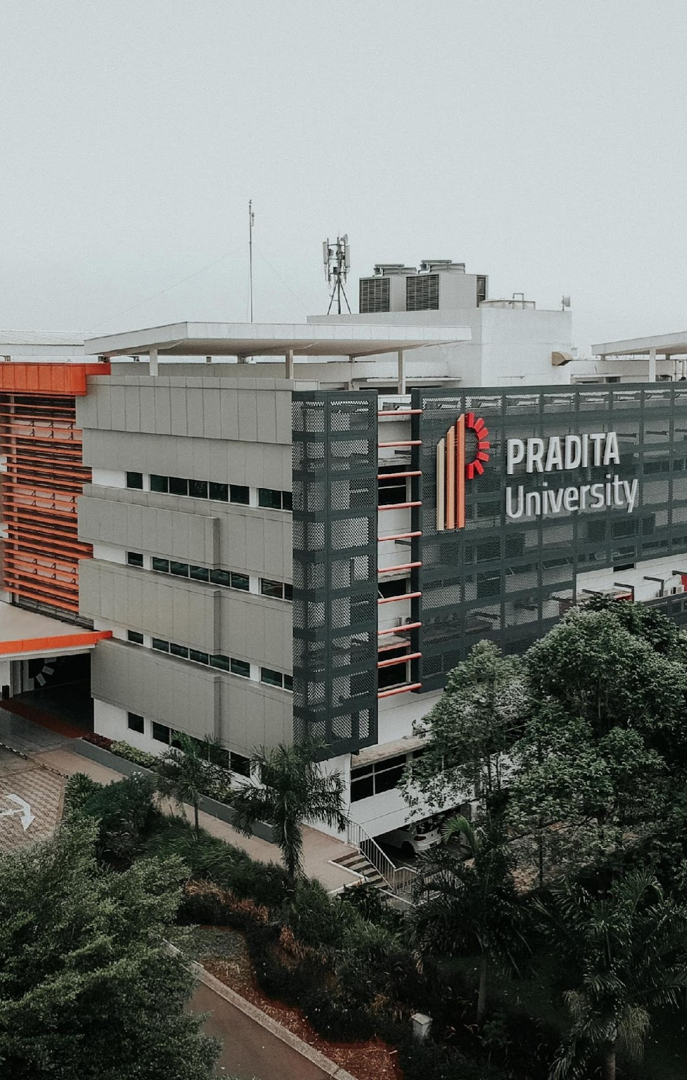
\includegraphics[width=\paperwidth, height=\paperheight, keepaspectratio=false]{../figures/building.png}
  };

  % --- Logo universitas: ditempatkan di tengah, dekat sisi atas ---
  \node[anchor=north, inner sep=0pt]
    at ([yshift=-0.10\paperheight] current page.north) {
    
\includegraphics[width=0.30\paperwidth]{../figures/logo_universitas.png}
  };

  % --- Blok judul: benar-benar di tengah halaman ---
  \node[anchor=center, align=center]
    at ([yshift=0.02\paperheight] current page.center) {
    \begin{minipage}{0.85\paperwidth}
      \centering
      {\LARGE \textbf{Modul Mata Kuliah IT30713}}\\[0.030\paperheight]
      {\HUGE \textcolor{praditagreen}{\textbf{Enterprise}}}\\[0.012\paperheight]
      {\HUGE \textcolor{praditagreen}{\textbf{\&}}}\\[0.012\paperheight]
      {\HUGE \textcolor{praditagreen}{\textbf{Platform Architecture}}}\\[0.050\paperheight]
      {\LARGE \textbf{Alfa Yohannis}}
    \end{minipage}
  };

  % --- Footer: pita hijau penuh selebar halaman, menempel di tepi bawah ---
  \node[
    anchor=south,
    fill=praditagreen,
    text=white,
    minimum width=\paperwidth,
    minimum height=0.13\paperheight,
    align=center,
    font=\Large\bfseries,
    inner sep=0pt
  ] at (current page.south) {%
    \begin{minipage}{0.9\paperwidth}
      \centering
      Program Studi Teknologi Informasi\\[4pt]
      Pradita University
    \end{minipage}%
  };

\end{tikzpicture}
\end{titlepage}
